% SGA 3, Exposé IX, tradução brasileira.
% Escopo: título e §1 integral.
% Autoridade: Polo--Gille Exp9-8nov09.pdf, pp. locais 1--3,
% leitor completo pp. 647--649, pp. impressas 37--40.
% O TeX inglês serve unicamente para o alinhamento estrutural; o PDF francês
% controla o texto, as fórmulas, a numeração e as notas.

\setcounter{footnote}{-1}
\SGARefTarget{sga3:ix:chapter:ix}\chapter*{Exposé IX\\
Grupos de tipo multiplicativo:\\
Homomorfismos em um esquema em grupos}
\addcontentsline{toc}{chapter}{Exposé IX. Grupos de tipo multiplicativo:
homomorfismos em um esquema em grupos}
\markboth{EXPOSÉ IX. GRUPOS DE TIPO MULTIPLICATIVO I (HOMOMORFISMOS)}
  {EXPOSÉ IX. GRUPOS DE TIPO MULTIPLICATIVO I (HOMOMORFISMOS)}

\begin{center}
  \textit{por A. Grothendieck}\footnote{Nota do editor: versão 1.0 de
  8 de novembro de 2009. Fizeram-se acréscimos na demonstração de
  \SGARefLink{sga3:ix:theorem:3:6:bis}{3.6 bis}, em
  \SGARefLink{sga3:ix:lemma:4:4}{4.4}--\SGARefLink{sga3:ix:theorem:4:7}{7},
  \SGARefLink{sga3:ix:lemma:5:0}{5.0}--\SGARefLink{sga3:ix:theorem:5:6}{6},
  \SGARefLink{sga3:ix:lemma:6:1}{6.1},
  \SGARefLink{sga3:ix:theorem:7:1}{7.1} e
  \SGARefLink{sga3:ix:proposition:8:2}{8.2}. Restam por revisar
  \SGARefLink{sga3:ix:proposition:8:1}{8.1} e
  \SGARefLink{sga3:ix:lemma:4:5}{4.5}.}
\end{center}

\SGARefTarget{sga3:ix:section:1}\section*{1. Definições}
\addcontentsline{toc}{section}{1. Definições}

% Página-fonte: Exp9 p. local 1; leitor completo p. 647; p. impressa 37.
\medskip
\noindent\SGARefTarget{sga3:ix:definition:1:1}\textbf{Definição 1.1.} ---
\textit{Seja \(S\) um pré-esquema e seja \(G\) um pré-esquema em grupos sobre
\(S\). Diz-se que o grupo \(G\) é \emph{de tipo multiplicativo} se for
localmente diagonalizável para a topologia fielmente plana e
quase compacta (cf.\ \SGARefLink{sga3:iv:subsection:6:3}{IV 6.3}); isto é,
se, para todo \(s\in S\), existem uma vizinhança aberta \(U\) de \(s\) e um
morfismo fielmente plano e quase compacto \(S'\to U\) tais que}
\[
  G'=G\times_S S'
\]
\textit{seja um \(S'\)-grupo diagonalizável
(\SGARefLink{sga3:i:subsection:4-4}{I 4.4} e
\SGARefLink{sga3:viii:definition:1:1}{VIII 1.1}).}

\textit{Diz-se que o grupo \(G\) é \emph{de tipo multiplicativo
quase-isotrivial} se for localmente diagonalizável até mesmo para a topologia
étale (\SGARefLink{sga3:iv:subsection:6:3}{IV 6.3}); isto é, se, na
definição precedente, se puder tomar \(S'\to U\) étale e sobrejetivo. De
maneira equivalente ---como se vê tomando a união disjunta dos esquemas
\(S'\) associados aos diversos \(s\in S\)---, existe um morfismo étale
sobrejetivo \(S'\to S\) tal que \(G'=G\times_S S'\) seja um \(S'\)-grupo
localmente diagonalizável.}

\textit{Se, além disso, for possível escolher \(S'\to S\) finito, étale e
sobrejetivo, diz-se que \(G\) é \emph{de tipo multiplicativo
isotrivial}.}

\textit{Por fim, diz-se que \(G\) é um grupo \emph{de tipo
multiplicativo localmente trivial} (respectivamente, \emph{de tipo
multiplicativo localmente isotrivial}) se todo \(s\in S\) possuir uma vizinhança
aberta \(U\) tal que \(G\times_S U\) seja um \(U\)-grupo diagonalizável
(respectivamente, seja de tipo multiplicativo isotrivial; dito de outro
modo, existe um morfismo finito étale sobrejetivo \(S'\to U\) tal que
\(G\times_S S'\) seja um \(S'\)-grupo diagonalizável).}

\medskip
\noindent\SGARefTarget{sga3:ix:comments:1:2}\textbf{Comentários 1.2.} ---
As cinco noções precedentes são todas obtidas, por localização, a partir
da noção de grupo diagonalizável, com respeito a cinco «topologias»
distintas associadas a \((\mathbf{Sch})\).

Subentende-se, em geral, que, quando a palavra «localmente» não é
precisada pelo nome da topologia considerada, trata-se da topologia de
Zariski, em conformidade com a terminologia estabelecida. Na terminologia
aqui introduzida, «de tipo multiplicativo localmente trivial» equivale a
«localmente diagonalizável» em
\SGARefLink{sga3:viii:definition:1:1}{VIII 1.1}; do mesmo modo, «trivial»
traduz-se por «diagonalizável». As cinco noções introduzidas se dispõem no
diagrama de implicações seguinte, que resulta das relações correspondentes
entre as topologias consideradas:

% Página-fonte: Exp9 p. local 2; leitor completo p. 648; pp. impressas 38--39.
\SGARefTarget{sga3:ix:diagram:1:2}
\begin{center}
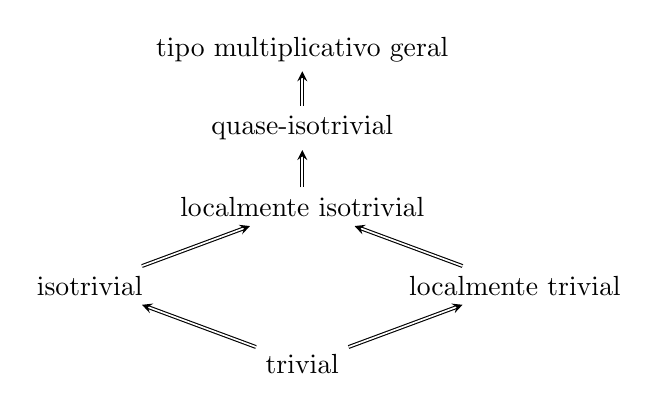
\begin{tikzpicture}[>=stealth]
  \node (general) at (0,4.0) {tipo multiplicativo geral};
  \node (quasi) at (0,3.0) {quase-isotrivial};
  \node (lociso) at (0,2.0) {localmente isotrivial};
  \node (iso) at (-2.7,1.0) {isotrivial};
  \node (loctriv) at (2.7,1.0) {localmente trivial};
  \node (triv) at (0,0) {trivial};
  \draw[double,->] (quasi) -- (general);
  \draw[double,->] (lociso) -- (quasi);
  \draw[double,->] (iso) -- (lociso);
  \draw[double,->] (loctriv) -- (lociso);
  \draw[double,->] (triv) -- (iso);
  \draw[double,->] (triv) -- (loctriv);
\end{tikzpicture}
\end{center}

Para as aplicações, assinalemos desde já que todo grupo de tipo
multiplicativo que encontrarmos será quase-isotrivial. Com efeito, veremos na
exposição seguinte (\SGARefLink{sga3:x:corollary:4-5}{X 4.5}) que,
quando \(G\) é de tipo finito sobre \(S\), ele é automaticamente
quase-isotrivial; daremos, contudo, exemplos nos quais não é localmente
isotrivial. Veremos igualmente que \(G\) pode ser localmente trivial sem ser
isotrivial e, portanto, \emph{a fortiori}, sem ser trivial. Daí se
deduz facilmente que as inclusões do
\SGARefLink{sga3:ix:diagram:1:2}{diagrama precedente} são estritas.

Por outro lado, veremos também ali
(\SGARefLink{sga3:x:theorem:5-16}{X 5.16}) que, se \(S\) é localmente
noetheriano e normal ---ou, mais geralmente, geometricamente
unirramoso---, todo grupo de tipo multiplicativo e de tipo finito sobre
\(S\) é necessariamente isotrivial; além disso, é trivial assim que for
localmente trivial (ou mesmo meramente trivial sobre um aberto denso).
Isso explica por que a maioria dos grupos de tipo multiplicativo que
aparecem na prática será, sem dúvida, isotrivial, tanto mais que
veremos adiante que os toros maximais dos esquemas em grupos
semissimples são automaticamente isotriviais.

\medskip
\noindent\SGARefTarget{sga3:ix:definition:1:3}\textbf{Definição 1.3.} ---
\textit{Sejam \(S\) e \(G\) como em
\SGARefLink{sga3:ix:definition:1:1}{1.1}. Chama-se \emph{toro} o grupo
\(G\) se, para a topologia fielmente plana e quase compacta, ele for localmente
isomorfo a um grupo da forma \(\mathbf G_m^r\), onde \(r\) é um
inteiro tal que \(r\geq0\).}

Com as notações de \SGARefLink{sga3:ix:definition:1:1}{1.1}, isso
significa que se pode escolher \(S'\) de modo que \(G'\) seja isomorfo a um
grupo da forma \((\mathbf G_{m,S'})^r\). O inteiro \(r\) depende de
\(s\in S\): é a dimensão da fibra
\[
  G_s=G\otimes_S\kappa(s).
\]
É uma função localmente constante de \(s\), como se vê imediatamente.
Essa observação deve ser generalizada da maneira seguinte.

% Página-fonte: Exp9 p. local 3; leitor completo p. 649; pp. impressas 39--40.
\medskip
\noindent\SGARefTarget{sga3:ix:definition:1:4}\textbf{Definição 1.4.} ---
\textit{Seja \(G\) um esquema em grupos diagonalizável sobre um corpo
\(k\). Assim, \(G\) é isomorfo a um grupo \(D_k(M)\), onde \(M\) é um
grupo comutativo ordinário determinado, a menos de isomorfismo, por essa
condição; mais precisamente,}
\[
  M\simeq\operatorname{Hom}_{k\text{-}\mathrm{gr}}
    (G,\mathbf G_{m,k})
\]
\textit{(\SGARefLink{sga3:viii:corollary:1:3}{VIII 1.3}). A classe de
isomorfismo de \(M\) chama-se o \emph{tipo} do grupo diagonalizável
\(G\); ela é manifestamente invariante por extensão do corpo de base.}

\textit{Seja agora \(G\) um esquema em grupos de tipo multiplicativo sobre
um pré-esquema qualquer \(S\). Para todo \(s\in S\), existe uma extensão
\(k\) de \(\kappa(s)\) tal que
\(G\times_S\operatorname{Spec}(k)\) seja um \(k\)-grupo
diagonalizável.\footnote{Nota do editor: com efeito, por hipótese existem
uma vizinhança aberta \(U\) de \(s\) e um morfismo fielmente plano e
quase compacto \(S'\to U\) tais que \(G_{S'}\) é diagonalizável. Para todo
\(s'\in S'\) sobre \(s\), o corpo \(\kappa(s')\) é uma extensão de
\(\kappa(s)\), e
\(G_{s'}=G\times_S\operatorname{Spec}(\kappa(s'))\) é diagonalizável.}
Seu tipo independe da extensão escolhida, pela observação
precedente, e chama-se o \emph{tipo de \(G\) em \(s\)}, ou o \emph{tipo
de \(G_s\)}. Em particular, se o próprio \(G\) é diagonalizável e, portanto,
isomorfo a um grupo da forma \(D_S(M)\), então, para todo \(s\in S\),
o tipo de \(G\) em \(s\) é a classe de isomorfismo de \(M\).}

\textit{Mais geralmente, se \(G\) é um grupo de tipo multiplicativo
sobre \(S\) e \(M\) é um grupo comutativo ordinário, diz-se que \(G\)
é \emph{de tipo \(M\)} se for de tipo \(M\) em todo ponto \(s\in S\); de
maneira equivalente, se \(G\) for localmente isomorfo a \(D_S(M)\) para a
topologia fielmente plana e quase compacta.}

\medskip
\noindent\SGARefTarget{sga3:ix:remark:1:4:1}\textbf{Observação 1.4.1.}
\footnote{Nota do editor: acrescentou-se o número
\SGARefLink{sga3:ix:remark:1:4:1}{1.4.1} às observações seguintes,
para que pudessem ser citadas posteriormente.}
\SGARefTarget{sga3:ix:remark:1:4:1:item:a}\textit{a) Para um grupo \(G\)
de tipo multiplicativo sobre \(S\), a função}
\[
  s\longmapsto \text{el tipo de }G_s
\]
\textit{é localmente constante sobre \(S\). Com efeito, com as notações
de \SGARefLink{sga3:ix:definition:1:1}{1.1}, se \(G'\) é de tipo \(M\),
então \(G\) é de tipo \(M\) sobre a vizinhança \(U\) de \(s\). Por
conseguinte, \(S\) possui uma decomposição canônica como união disjunta de
pré-esquemas \(S_i\) tais que, para todo \(i\), \(G_{S_i}\) é de tipo
\(M_i\), onde os grupos comutativos \(M_i\) não são isomorfos dois a dois.}

\SGARefTarget{sga3:ix:remark:1:4:1:item:b}\textit{b) Em particular, se
\(S\) é conexo, o tipo das fibras de \(G\) é constante; isto é,
existe um grupo comutativo \(M\) tal que \(G\) é de tipo \(M\). Por
fim, se \(G\) é um toro, o tipo de \(G\) em \(s\) é determinado
pelo inteiro \(\dim G_s\): com efeito, \(G_s\) é de tipo \(\mathbb Z^n\),
onde \(n=\dim G_s\).}

\medskip
\noindent\SGARefTarget{sga3:ix:remark:1:5}\textbf{Observação 1.5.} ---
\SGARefTarget{sga3:ix:remark:1:5:item:a}\textit{a) Das Definições
\SGARefLink{sga3:ix:definition:1:1}{1.1} e
\SGARefLink{sga3:ix:definition:1:3}{1.3} segue imediatamente que essas
noções são «compatíveis com a extensão da base». Assim, se \(G\) é
um pré-esquema em grupos sobre \(S\) e \(S'\to S\) é um morfismo de mudança
de base, então, sempre que \(G\) for de tipo multiplicativo
(respectivamente, de tipo multiplicativo isotrivial etc.), o mesmo valerá
para \(G'\).}

\SGARefTarget{sga3:ix:remark:1:5:item:b}\textit{b) Se, além disso, \(S'\to S\)
é fielmente plano e quase compacto, o fato de \(G'\) ser de tipo
multiplicativo, respectivamente um toro, implica o mesmo para \(G\). Se
\(S'\to S\) também é étale (respectivamente, finito étale), o fato de
\(G'\) ser quase-isotrivial (respectivamente, isotrivial) implica o
mesmo para \(G\).}

\SGARefTarget{sga3:ix:remark:1:5:item:c}\textit{c) Voltemos, por fim, a
um morfismo de mudança de base qualquer \(f:S'\to S\). Se \(s'\in S'\) e
\(s=f(s')\), o tipo de \(G'\) em \(s'\) é o mesmo que o de \(G\) em
\(s\), pois}
\[
  G'_{s'}=G_s\otimes_{\kappa(s)}\kappa(s').
\]
